% !TEX TS-program = pdflatex
%% !TEX encoding = UTF-8 Unicode
% !TEX spellcheck = en_US

% This is a simple template for a LaTeX document using the "article" class.
% See "book", "report", "letter" for other types of document.

\documentclass[11pt]{paper} % use larger type; default would be 10pt

\usepackage{lineno}

\usepackage{setspace}
%\doublespacing

%%% Examples of Article customizations
% These packages are optional, depending whether you want the features they provide.
% See the LaTeX Companion or other references for full information.

%%% PAGE DIMENSIONS
%\usepackage{geometry} % to change the page dimensions
%\geometry{a4paper} % or letterpaper (US) or a5paper or....
% \geometry{margin=2in} % for example, change the margins to 2 inches all round
% \geometry{landscape} % set up the page for landscape
%   read geometry.pdf for detailed page layout information
\usepackage{mathtools}
\usepackage{graphicx} % support the \includegraphics command and options
\usepackage{caption}
\usepackage{subcaption}
\usepackage{wrapfig}
\usepackage[leftcaption]{sidecap}

\graphicspath{{./}{./fig/}}

\usepackage[style=numeric-comp, sorting=none, url=false, isbn=false]{biblatex}
\addbibresource{binding-pocket.bib}

% \usepackage[parfill]{parskip} % Activate to begin paragraphs with an empty line rather than an indent

%%% PACKAGES
%\usepackage{booktabs} % for much better looking tables
%\usepackage{array} % for better arrays (eg matrices) in maths
%\usepackage{paralist} % very flexible & customisable lists (eg. enumerate/itemize, etc.)
%\usepackage{verbatim} % adds environment for commenting out blocks of text & for better verbatim
%\usepackage{subfig} % make it possible to include more than one captioned figure/table in a single float
% These packages are all incorporated in the memoir class to one degree or another...

%%% HEADERS & FOOTERS
%\usepackage{fancyhdr} % This should be set AFTER setting up the page geometry
%\pagestyle{fancy} % options: empty , plain , fancy
%\renewcommand{\headrulewidth}{0pt} % customise the layout...
%\lhead{}\chead{}\rhead{}
%\lfoot{}\cfoot{\thepage}\rfoot{}

%%% SECTION TITLE APPEARANCE
%\usepackage{sectsty}
%\allsectionsfont{\sffamily\mdseries\upshape} % (See the fntguide.pdf for font help)
% (This matches ConTeXt defaults)

%%% ToC (table of contents) APPEARANCE
%\usepackage[nottoc,notlof,notlot]{tocbibind} % Put the bibliography in the ToC
%\usepackage[titles,subfigure]{tocloft} % Alter the style of the Table of Contents
%\renewcommand{\cftsecfont}{\rmfamily\mdseries\upshape}
%\renewcommand{\cftsecpagefont}{\rmfamily\mdseries\upshape} % No bold!

%%% END Article customizations

%%% The "real" document content comes below...

\title{Odorant receptors of \textit{Drosophila} are sensitive to molecular volume of odorants}
\author{Majid Saberi \and Hamed Seyed-allaei\thanks{hamed@ipm.ir}}
\institution{School of Cognitive Science, \\ Institute for Research in Fundamental Sciences (IPM), \\Tehran, Iran}
%Olfactory System; Odorant Receptor; Chemical Range; G Protein-Coupled Receptors; Odor-Structure Relation;
%Majid Saberi <majidsaberi048@gmail.com>
%leslie.vosshall@rockefeller.edu
%giovanni.galizia@uni-konstanz.de
%m.schmuker@biomachinelearning.net Michael Schmuker

%\date{} % Activate to display a given date or no date (if empty),
         % otherwise the current date is printed 

\newcommand{\numberofreceptors}{ 28 }
\newcommand{\bonferroni}{ 11 }
\newcommand{\fdr}{ 26 }
\newcommand{\nocorrection}{ 2 }

\begin{document}


%\linenumbers

\maketitle

\begin{abstract} 
Which properties of a molecule define its odor? This is a basic question of olfaction, 
yet to be answered. \textit{Drosophila}'s olfactory system has a repertoire of about 60 odorant receptors. 
Molecules bind to them with different affinities and activate them with different efficacies, 
resulting in a combinatorial code that identifies odorants. 
We hypothesized that the binding affinity between a pair of odorant-receptor is affected by their relative sizes. 
The affinity can reaches its maximum if molecular volume of an odorant matches volume of a receptor's binding-pocket 
and it reach zero if the sizes are too different, 
obscuring the effect of other molecular properties. 
We formulated this hypothesis mathematically and verified it on data of \textit{Drosophila}, 
and predicted the volume and the structural flexibility of each receptor's binding-site, 
which are significantly different among receptors. 
This provides a reason for differences in smell among similar molecules of different sizes. 
\end{abstract}



%\section*{Significance Statement}
%We perceive wavelength of light as its colors and frequency of sound as its pitch. But we don’t know yet what properties of molecules are perceived as smell. In this work, for the first time, we showed that molecular volume of an odorant is an important factor in the fruit fly. It affects two dimensions of smell: its intensity (weak or strong) and its quality (sweet, floral, fruity or etc). The molecular volume could describe the difference in the smell of methanol and butanol. Methanol smells pungent while butanol smells winy with a tad of banana like aroma.

\section*{Introduction}
\begin{figure}
	\centering
	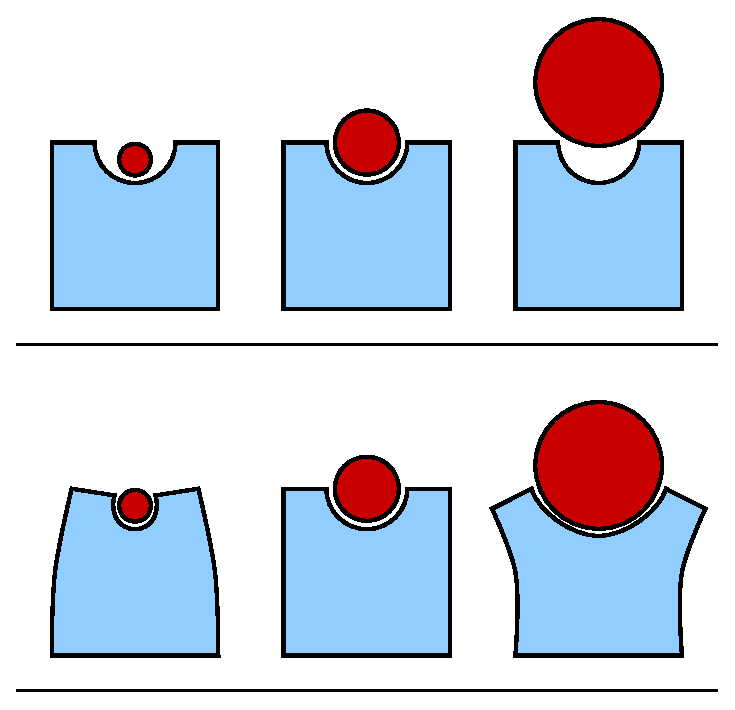
\includegraphics[width=0.4 \textwidth]{binding-pocket-size-flex}
	\caption{This figure shows different scenarios that may happen when an odorant molecule (ligand) binds to a receptor. 
		The red disks  are odorant molecule, 
		and the blue shapes are OR and binding-pocket.	
		(top) From left to right, misfit because of small volume of molecule, 
		perfect match and misfit because of large molecular volume.
		(down) The flexibility of a receptor may compensate for the volume mismatches.
		}
	\label{fig:binding-pocket}
\end{figure}

%Survival of many species depends on their olfactory system. 
%They use it  to find food, 
%avoid poison, 
%escape from danger, 
%mate, 
%and bind to their offspring.
%An olfactory system detects volatile chemicals in the surrounding, 
%encodes the results and transmit them to limbic system and cortex.

We know that which properties of light are measured by our eyes and how our eyes do that. 
That knowledge assisted the production of cameras and displays. 
Unfortunately we do not have the same knowledge in olfaction, 
we do not know the relation between the stimuli --molecular properties-- and sensory experiences --the quality of smells.  

%Molecules of a volatile material evaporates into air, 
%the concentration of the vapor depends on the vapor pressure of the material and its temperature, 
%the vapor reaches sensilla of the insect (epithelium in human), 
%depending on their solubility in water, they enter sensillum lymph (mucosa in human), 
%and the odorant binding protein may also help them to reach odorant receptor neurons (ORNs) and bind to their odorant receptors (ORs). 

The front end of the olfactory system are olfactory receptor neurons (ORNs).  
Each ORN expresses only one kind of OR. 
% (in insects many are co-expressed with Orco \cite{Larsson2004}).
ORN of the same kind converge into the same glomeruli of antennal lobe in insects (or olfactory bulb in human)
%so that each glomerulus receives an amplified signal from only one type of OR
~\cite{root2007,Carey2011,Vosshall2000,Couto2005,fishilevich2005,gao2000,wang1998,mombaerts1996,vassar1994}.
%That makes the olfactory bulb (or antennal lobe in insects) the target of methods like calcium imaging (eg. ~\cite{Silbering2012}), 
%whereas electro-physiological studies directly target olfactory receptor neurons (eg.~\cite{Benton2010}). 

The olfactory system uses a combinatorial code: 
unlike many other receptors which are activated by only one specific ligand -- a neurotransmitter or a hormone,
an OR can be triggered by many odorant molecules, 
and an odorant molecule can interact with different OR types~\cite{Malnic2000},
The combinatorial code enables humans to discriminate many odors~\cite{Bushdid2014} by using a repertoire of only about 350 ORs.
However, it is not clear yet which properties of a molecule contribute to its smell. 
It is a topic of ongoing researches and there are many theories~\cite{Turin,Keller2004,Araneda2000,Brookes2007,Franco2011,Pelz2006,Gabler2013,Schmuker2007,Haddad2008,Snitz2013,Yablonka2012,gane2013}.

The ORs are transmembrane proteins, 
in insects they are ionotropic~\cite{Sato2008,Wicher2008,Nagel2011,Rong2011}, 
their topology is different from vertebrates~\cite{Benton2006,Smart2008},
and most of them function in presence of another common receptor, called Orco~\cite{Larsson2004}.
In vertebrates, they are metabotropic receptors, they belong to the family of g-protein coupled receptor (GPCR). 

There are many similarities between the olfactory system of insects and vertebrates~\cite{Wilson2014,Kaupp2010}.
Regardless of the signal transduction, 
all ORs have the same function, they have a binding-pocket (also known as binding-cavity and binding-site),
where odorants (ligands) bind to. 
Binding to an odorant activates an OR and 
the activated OR changes the potential of the cell, 
directly (ionotropic in insects) or indirectly (metabotropic in vertebrates);
Therefore, what we learn from olfactory system of \textit{Drosophila} can help us to decode human olfaction. 

%and it was assumed that insects use the same kind of signal transduction~\cite{Brody2000,Hill04102002}. 

The amount of change in the membrane potential of an ORN depends on the number of activated ORs and the time that they remain activated,
which are determined by various physio-chemical properties of the odorant and the OR~\cite{Turin,Araneda2000,Gabler2013,guerrieri2005,uchida2000}.
One important factor is the relative size of the ligand and the OR's binding pocket, 
it has been used in computational drug design as predictor of binding pocket for a given ligand~\cite{liang1998anatomy}. 
Another factor is the flexibility of the binding pocket, 
proteins are not rigid bodies,  
and they can change shape, 
depending on the amino acids involved~\cite{Ramachandran,apostolakis1998docking,gunasekaran2007different}.

Therefore, here we focused on the volume and the flexibility of the binding-pocket.
The molecular volume of a ligand should match the dimensions of the binding-pocket of the OR,
then it fits into the binding-pocket of the OR and triggers the signal transduction. 
Any mismatch in the volume will decrease the neural responses, 
on the other hand the flexibility of the binding-pocket can compensate for the volume mismatch (Fig. \ref{fig:binding-pocket}).

We could know the volume and flexibility of the binding-pocket, 
if we knew its three dimensional structure. 
But this is not the case here, 
as it is not easy to know the structure of integral proteins~\cite{Zhang2008,Lupieri2009}, 
including ORs. 
This is the topic of ongoing researches, 
using various methods like Molecular Dynamic (MD) simulations, 
mutagenesis studies, heterologus expression studies, and homology modeling~\cite{Khafizov2007,Man2004,Lai2005,Vaidehi2002,Floriano2004,Schmiedeberg2007,Katada2005,Kato2008,Rospars2013}.

In this study, 
we develop a mathematical framework to put the available experimental data in the best use and
investigated the relation between molecular volumes of odorants and the responses of ORNs. 
Our results suggest that molecular volume is a considerable factor, 
but not the only factor that determines the neural response of the ORNs.
We predicted the {\it in-vivo} volume and flexibility of binding-pocket of ORs (supplemental file volume-profiles.csv), 
by applying our mathematical method to neural data from DoOR database~\cite{Galizia2010}. 
it is a well structured database that includes the neural responses of most ORs of \textit{Drosophila} to many odorants~\cite{Galizia2010}. 
This database aggregated data from many sources~\cite{Bruyne1999,Bruyne2001,Dobritsa2003,Goldman2005,Hallem2004,Hallem2006,
Kreher2005,Kreher2008,Kwon2007,Pelz2006,Pelz2006,Schmuker2007,Stensmyr2003,
Turner2009,VanderGoesvanNaters2007,Yao2005}.

We suggested a functional relation between molecular volume and the neural responses, 
we provided a methodology to estimate {\it molecular receptive range} or {\it tuning function} of ORs,
and then we predicted the structural properties of the binding-pocket of OR - the volume and the flexibility of binding-pocket.
Our results may help to select odorants  for new experimental studies (supplemental file proposed-odorants.csv), 
%may provide additional information about the structure of ORs to structural biologists, 
and may contribute to the study of olfactory coding by unmasking the effect of other possible factors.

%%
%There are many studies that tries to connect physio-chemical properties of molecules to their perceived smells, like the current work, which studies the effect of molecular volume of odorants on the response of odorant receptors.

%The olfactory system of insects are similar to the olfactory system of vertebrates in many ways ...  However, there are also differences .... 

%Some receptors respond to few molecules, some response to many.

%Insects receptors neurons show spontaneos activity of 8 Hz.

%Drosophila's odorant receptors are ionotropic. They may be metabotropic. It is under debate.

% They have seven trans-membrane domains. They need Or83b to work. 
% they may construct a complex that work as a cation channel or Or83b functions as cation channel and collaborte with odorant receptor.

% odorant receptor are presents in other organs like kindny ans sperms.

%chemical receptory range.

%in GPCR odorant interact with helix 2,7
%2-58 candidate residues.

%Drosophila about 60 receptors, mamals 300-1300 receptors. 

%In low concentraiotn the response is narrow. In high concentration the response is broad.

%OR67d Pheremone. 
%Odor prediciton from the shape.
%Olfactory white.


%we show that the Drosophila melanogaster male-specific pheromone 11-cis-vaccenyl acetate (cVA) acts through the receptor Or67d to regulate both male and female mating behaviour. ~\cite{Kurtovic2007}
%we show that a Drosophila melanogaster CD36 homologue, Sensory neuron membrane protein (SNMP), is expressed in a population of olfactory sensory neurons (OSNs) implicated in pheromone detection.~\cite{Benton2007}
 
%we find that Drosophila ORs and OR83b adopt a novel membrane topology with their N-termini and the most conserved loops in the cytoplasm.~\cite{Benton2006}

%We find that major components of olfaction, including olfactory receptors (ORs), olfactory-related adenylate cyclase (AC3) and the olfactory G protein (G olf), are expressed in the kidney.~\cite{Pluznick2009}
 
%Most Drosophila olfactory neurons express two types of odorant receptor genes: Or83b, a broadly expressed receptor of unknown function, and one or more members of a family of 61 selectively expressed receptors.~\cite{Larsson2004}
 
%Humans can discriminate several million different colors and almost half a million different tones,On the basis of the results of psychophysical testing, we calculated that humans can discriminate at least 1 trillion olfactory stimuli.~\cite{Bushdid2014}

\section*{Material and methods}
\begin{figure}
	\centering
	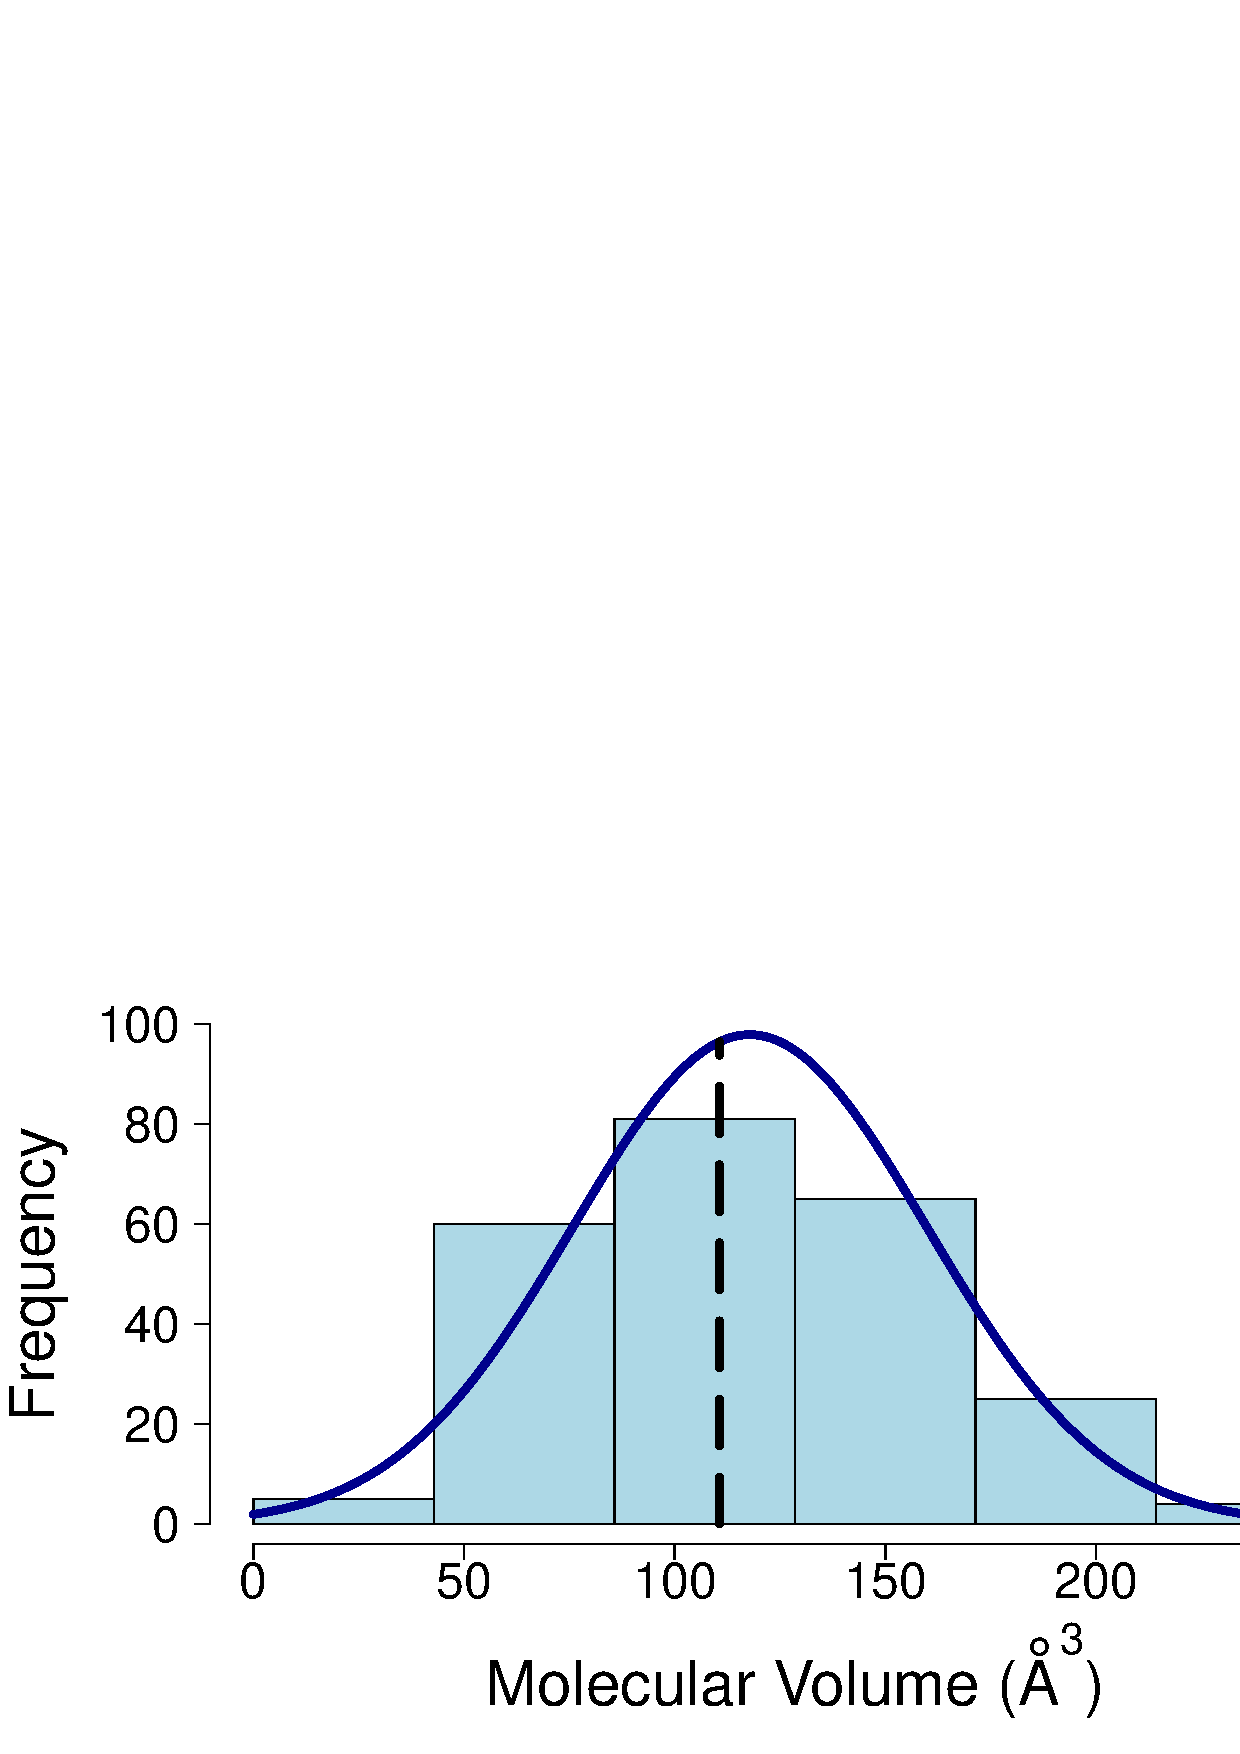
\includegraphics[width=0.5 \textwidth]{hist-volumes}
	\caption{Density function of molecular volumes $g(v)$, considering all molecules of DoOR database. 
		%The actual density function of molecular of volumes in each experiment, $g(v)$, might be slightly different  because each experiment uses a different subset of molecules. 
		The solid line is a Gaussian fit (Eq. \ref{eqn:hist-volumes}) and the dashed line shows the median, 
		which is slightly different from  the mean.}
	\label{fig:hist-volumes}
\end{figure}
%We studied the relation between neural responses and molecular volumes, 
We took the neural data of DoOR 1.0 database \cite{Galizia2010}, hold out  the additional data of DoOR 2.0 as a test set \cite{}. 
We calculated molecular volume (supplemental file odorants.csv) using a computational chemistry software -- VEGA ZZ~\cite{Pedretti2004}. 
We used  GNU R to analyze the data~\cite{Rlanguage}.

DoOR database includes an $N\times M$ matrix. 
Its elements, $r_{nm}$, are the response of neuron $n$ to odorant $m$. 
This matrix is normalized between 0 and 1 so $0 \le r_{nm} \le 1$, where 1 is the strongest response.
This matrix has many {\it Not Available} (NA) values, 
and different neurons are excited by different set of odorants, 
we took care of this by removing NAs from the summations and calculating $\sum_{m: r_{nm} \neq \text{NA}}$, 
but for brevity, we used the usual notation $\sum_m$.

The response $r_{nm}$ may depends on the molecular volume of the odorant, $v_m$, 
and other physio-chemical properties of the molecule $m$; 
we separated the response $r_{nm}$ into two terms:

\begin{equation}
	r_{nm} = f_n(v_m) \psi_{nm}.
	\label{eqn:factors}
\end{equation}
The first term, $f_n(v_m)$, depended only on the molecular volume of odorants.
The second term, the volume independent term $\psi_{nm}$, included every other influential properties of molecules, 
but the molecular volume or any other properties that correlates to molecular volume (eg, molecular weight).
Among all the molecular parameter that correlate with molecular volume, 
we used molecular volume because it  fits to the acceptable picture of protein-ligand interaction \cite{fig:binding-pocket}.

Both terms were characteristic of each OR, and they varied from OR to OR.
In fact, the first term, $f_n(v)$, can be considered as the tuning curve of neuron $n$ in respect to the molecular volumes. 
To keep the calculation simple, we approximated it with a Gaussian function,  

\begin{equation}
	\displaystyle f_n(v) = e^{-\frac{(v-v_n)^2}{2\sigma^2_n}}, 
	\label{eqn:volume-dependence}
\end{equation}
where, $v_n$ was the preferred molecular volume of OR $n$ and $\sigma_n$ represented its flexibility. 
In this work we wanted to estimate $v_n$ and $\sigma_n$. 
To do so, first we calculated the response weighted average of molecular volumes, 
$\frac{\sum_{m} v_m r_{nm}}{\sum_{m} r_{nm}}$ and then we use (\ref{eqn:factors}):

\begin{equation}
	\frac{\displaystyle \sum_{m} v_m r_{nm}}{\displaystyle \sum_{m} r_{nm}} = \frac{\displaystyle \sum_{m} v_m f_n(v_m) \psi_{nm}}{\displaystyle \sum_{m} f_n(v_m) \psi_{nm}}.
	\label{eqn:sta}
\end{equation}
We approximated $\sum$ with $\int$, which is common in statistical physics:

\begin{equation}
	\sum_{m} \dots f_n(v_m) \psi_{nm} \approx  \langle \psi_{nm} \rangle_m \int_0^\infty \dots f_n(v) g(v)  dv. 
	\label{eqn:sigma_to_int}
\end{equation}
In which, 
$\langle \psi_{nm} \rangle_m$ denoted the average of $\psi_{nm}$ over all $m: r_{nm} \neq \text{NA}$. 
We moved out of the integral for it was independent of $v$.
Here $g(v)$ was the density of states, $g(v) dv$ indicated how many molecules have a molecular volume in the range of $v$ and $v+dv$.
This function was approximated by a Gaussian function (Fig.~\ref{fig:hist-volumes}), 

\begin{equation}
	g(v) = e^{-\frac{(v- v_{g})^2}{2 \sigma_{g}^2}},
	\label{eqn:hist-volumes}
\end{equation}
ideally, $g(v)$ must not depend on the OR $n$ for it is the property of ensemble of odorant molecules, not ORs. 
But here, we had many missing values ($r_{nm} = NA$) that were not overlapping, 
so we had to calculate $g(v)$ for each neuron separately; 
Therefore, $v_{g_n}$ and $\sigma_{g_n}$ were the average and standard deviation of molecular volume while $r_{nm} \neq \text{NA}$.
We rewritten equation (\ref{eqn:sta}) using equation (\ref{eqn:sigma_to_int}):

\begin{equation}
	\frac{\displaystyle \sum_{m} v_m r_{nm}}{\displaystyle \sum_{m} r_{nm}} \approx \frac{\displaystyle \int v f_n(v) g_n(v) dv}{\displaystyle \int f_n(v) g_n(v) dv}.
	\label{eqn:sta_int}
\end{equation}
We replaced the product of $f_n(v)$ and $g_n(v)$ in the above equation with $h_n(v) = f_n(v) g_n(v)$, to make a simpler form

\begin{equation}
	\frac{\displaystyle \sum_{m} v_m r_{nm}}{\displaystyle \sum_{m} r_{nm}} \approx \frac{\displaystyle \int_v v h_n(v) dv}{ \displaystyle \int_v  h_n(v) dv }.
	\label{eqn:mean}
\end{equation}
The function $h_n(v)$ was a Gaussian function for it was the product of two Gaussian functions, 

\begin{equation}
h_n(v) = e^{-\frac{(v-\mu_{h_n})^2}{2\sigma_{h_n}^2}}, 
\end{equation}
so the right hand side of equation \ref{eqn:mean} was nothing but $\mu_{h_n}$ and 
in a similar way, we calculated $\sigma_{h_n}$ from the neural data

\begin{eqnarray}
	\mu_{h_n} &\approx& \frac{\displaystyle \sum_{m} v_m r_{nm}}{\displaystyle \sum_{m} r_{nm}} \\
	\sigma_{h_n}^2 &\approx& \frac{\displaystyle \sum_{m} v_m^2 r_{nm}}{\displaystyle \sum_{m} r_{nm}} - \mu_{h_n}^2
	\label{eqn:final_h}
\end{eqnarray}


We knew the mean, $v_{g_n}$, and standard deviation, $\sigma_{g_n}$, of $g_n(v)$ from the molecular volumes of the ensembles of odorants. 
We calculated the mean $\mu_{h_n}$ and standard deviation $\sigma_{h_n}$ of $h_n(v)$ from the neural data.
Using them, we calculated the mean $v_n$ and the standard deviation $\sigma_n$ of $f_n(v)$:
first we calculated $\sigma_n$ from 

\begin{equation}
	\frac{1}{\sigma_n^2} = \frac{1}{\sigma^2_{h_n}}  - \frac{1}{\sigma^2_{g_n}}
\end{equation}
and then we calculated $v_n$: 

\begin{equation}
	\frac{v_n}{\sigma_n^2}  =    \frac{\mu_{h_n}}{\sigma^2_{h_n}} - \frac{v_{g_n}}{\sigma^2_{g_n}}.
\end{equation}
The calculated $v_n$ and $\sigma_n$ were put in supplemental file volume-profiles.csv. 
The resulting $f_n(v)$ were plotted over the actual data, for \numberofreceptors ORs (Fig.~\ref{fig:vol-res}),
in which p-values $<0.05$. 

We calculated p-values by permutation test, shuffling the data $10^5$ times. 
We shuffled the association between odorants and responses of a given OR,  
and then check the null and alternative hypothesis. 
The alternative hypothesis was
``{\it The response of ORN depend on the molecular volume of odorants.}'', 
which required  a finite value for $\sigma_n$, 
then the null hypothesis was 
``{\it The response of ORN is independent of molecular volume of odorants.}'',
which required $\sigma_n \rightarrow \infty$, 
so p-value was the probability of having $\sigma'_n\leq\sigma_n$, 
where $\sigma_n$ was calculated from the original data, but $\sigma'_n$ was calculated using permuted version. 

We were testing a hypothesis on $\sim$60 ORs simultaneously. 
If we had used a simple threshold of 0.05 for the p-value of each OR, we could had have many false positives. 
To address this issue, multiple-comparison problem, 
we used Bonferroni correction (we multiply p-values by 60). 
The problem with Bonferroni correction is that it may increases false negatives.
This problem can be addressed using another method -- False Discovery Rate (FDR)--  that keeps the rate of false positive below a threshold \cite{benjamini1995controlling,shaffer1995multiple}.
We used both methods -- Bonferroni and FDR, as well as no correction. We used the function p.adjust of GNU R to calculate the corrected p-values. 
The result were labeled accordingly in Fig.~\ref{fig:vol-res}.

We also wanted to show the diversity of volume and flexibility of binding pocket among ORs.
To estimate the p-values, 
we took any pair of ORs that were sensitive to molecular volume (\numberofreceptors ORs),
calculate their difference, 
used a permutation test ($6\times10^4$ shuffles) and measured the probability of being different only by chance (Fig.~\ref{fig:p-values}).

%Now we know the preferred volume $v_n$ of each receptor and also its flexibility $\sigma_n$.

\section*{Results and discussions}
\begin{figure}
	\centering
%	\begin{subfigure}[b]{\textwidth}
		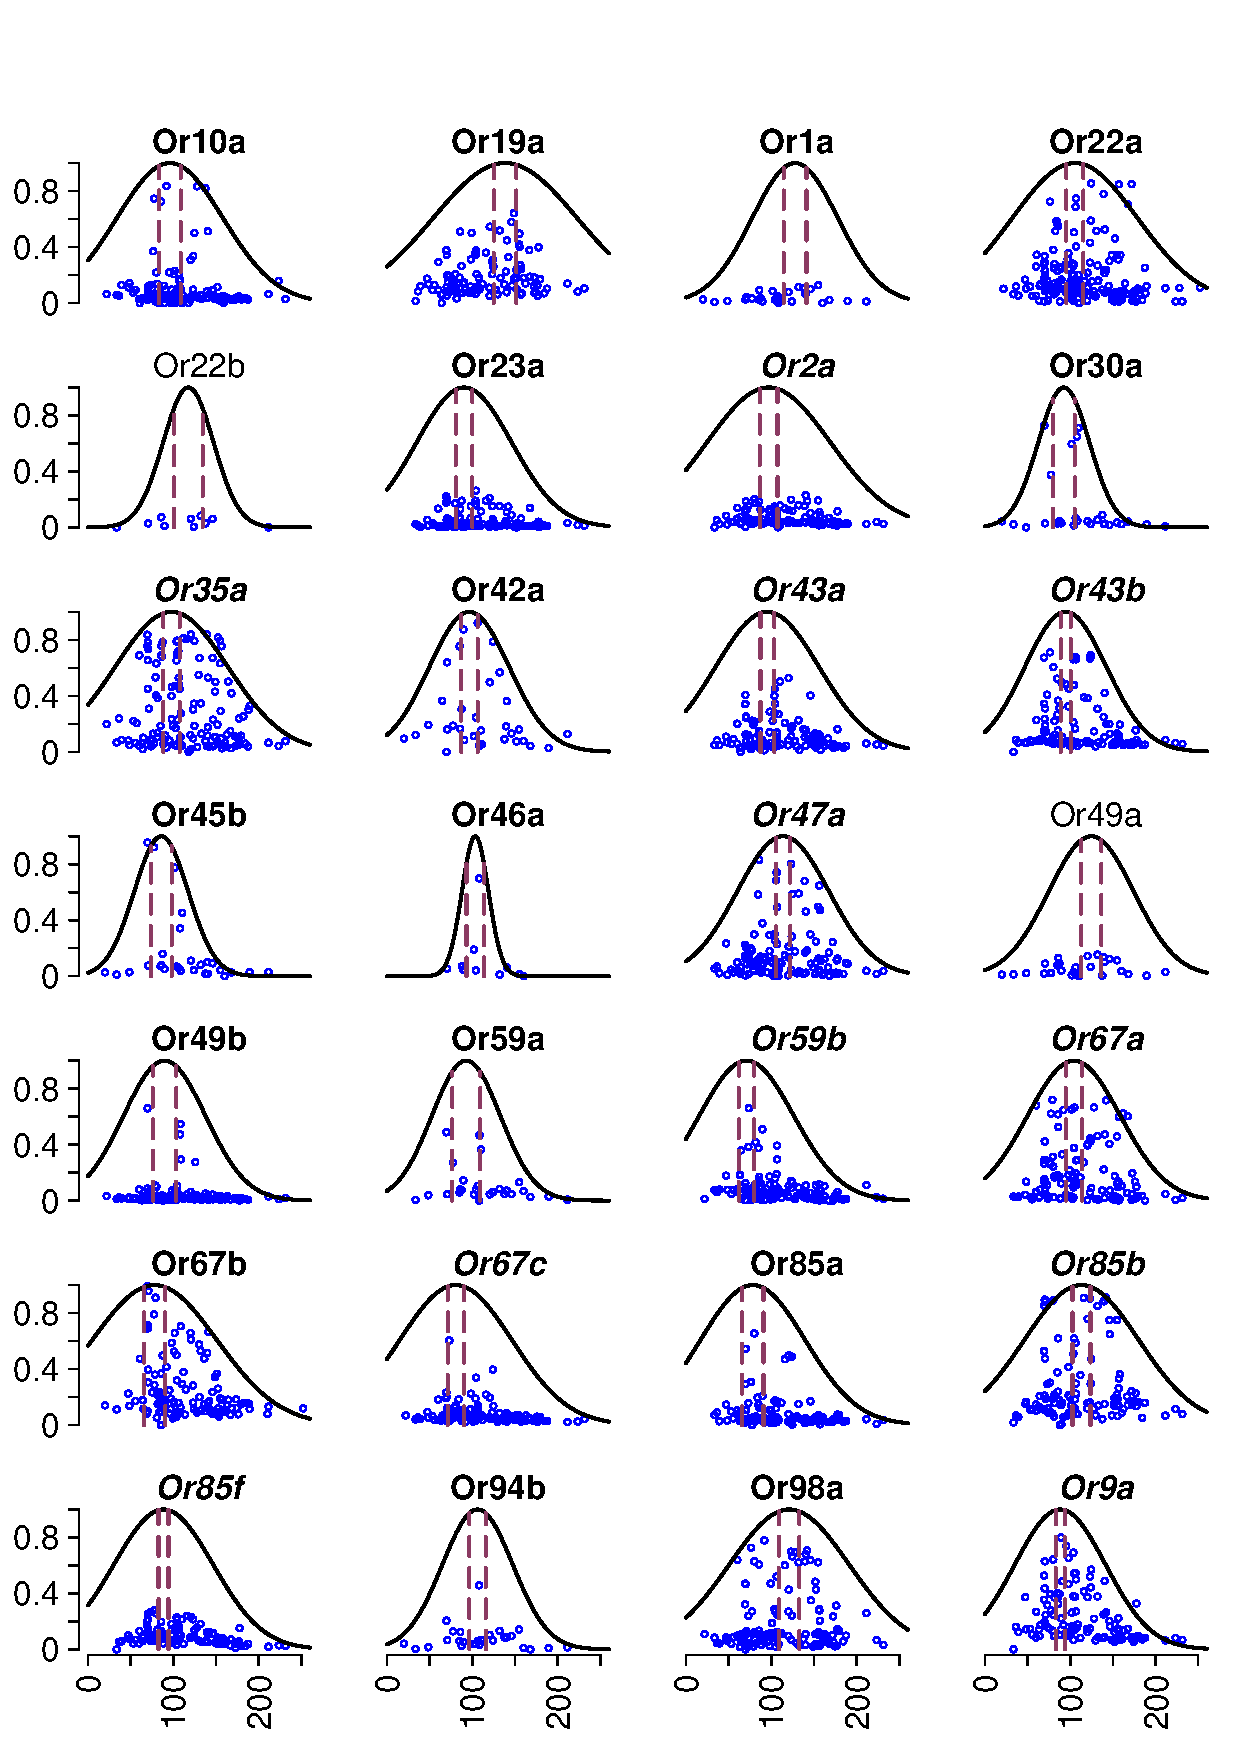
\includegraphics[width=0.8 \textwidth]{vol-res-}
		%\caption{}
		\label{fig:vol-res:all}		
%	\end{subfigure}
%	\begin{subfigure}[b]{0.75 \textwidth}
%		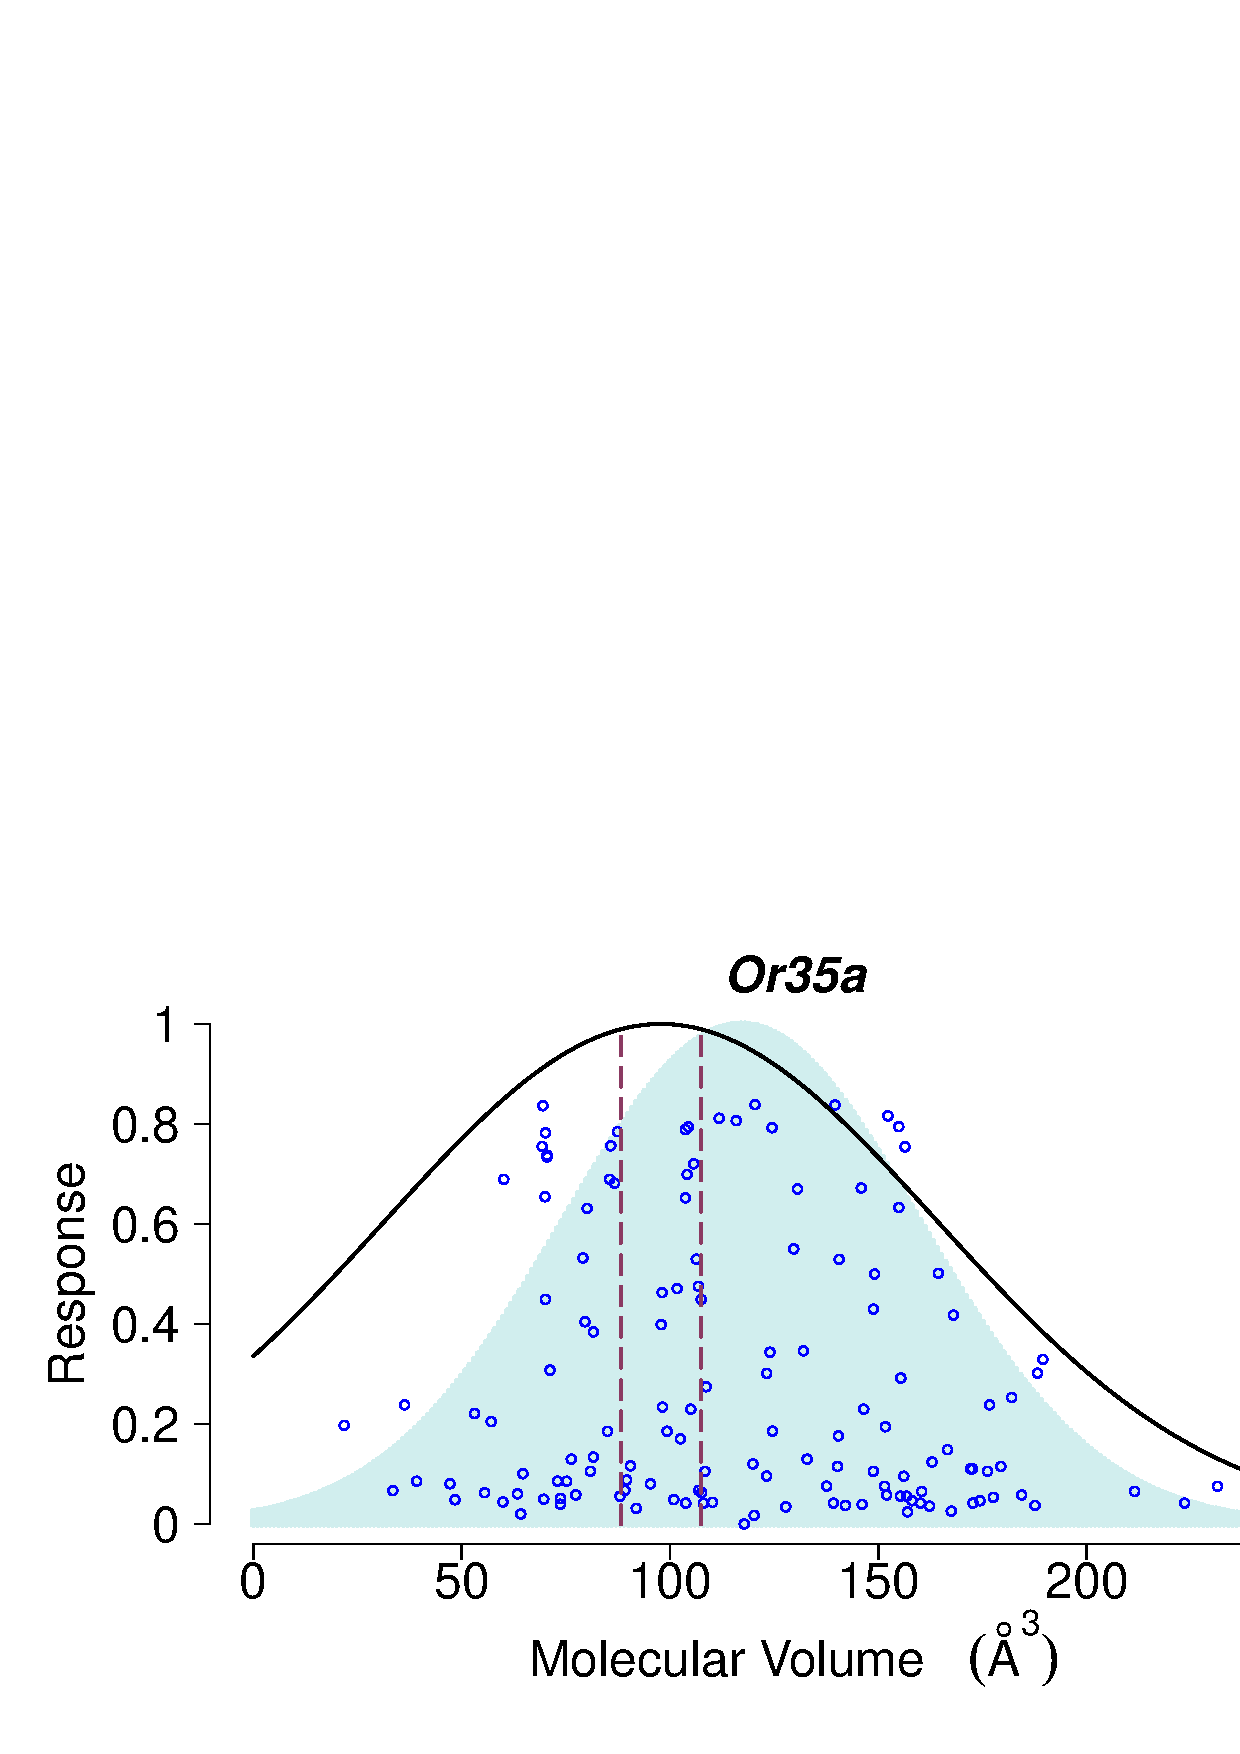
\includegraphics[width= \textwidth]{fig/vol-res-Or35a}
%		\caption{}	
%		\label{fig:vol-res:one}	
%	\end{subfigure}
	\caption{Response of ORs  versus molecular volume of odorants (circles),  
			the fitted functions $f_n(v)$ from Eq.~\ref{eqn:factors} (solid lines), 
			and the error bars of the mean of $f_n(v)$ (red vertical lines), 
			for \numberofreceptors ORs that their response showed significant (p-value $<0.05$) dependence to molecular volume. 
			Except one (OR name in light gray), \fdr were significant according to FDR correction (OR names in gray) and 
			\bonferroni were significant considering Bonferroni correction (OR names black).
			The function $f_n(v)$ was calculated based on data from DoOR 1.0 (blue circles), 
			The red circles are additional data of DoOR 2.0. 
		}
	\label{fig:vol-res}
\end{figure}

\begin{figure}
		\centering
		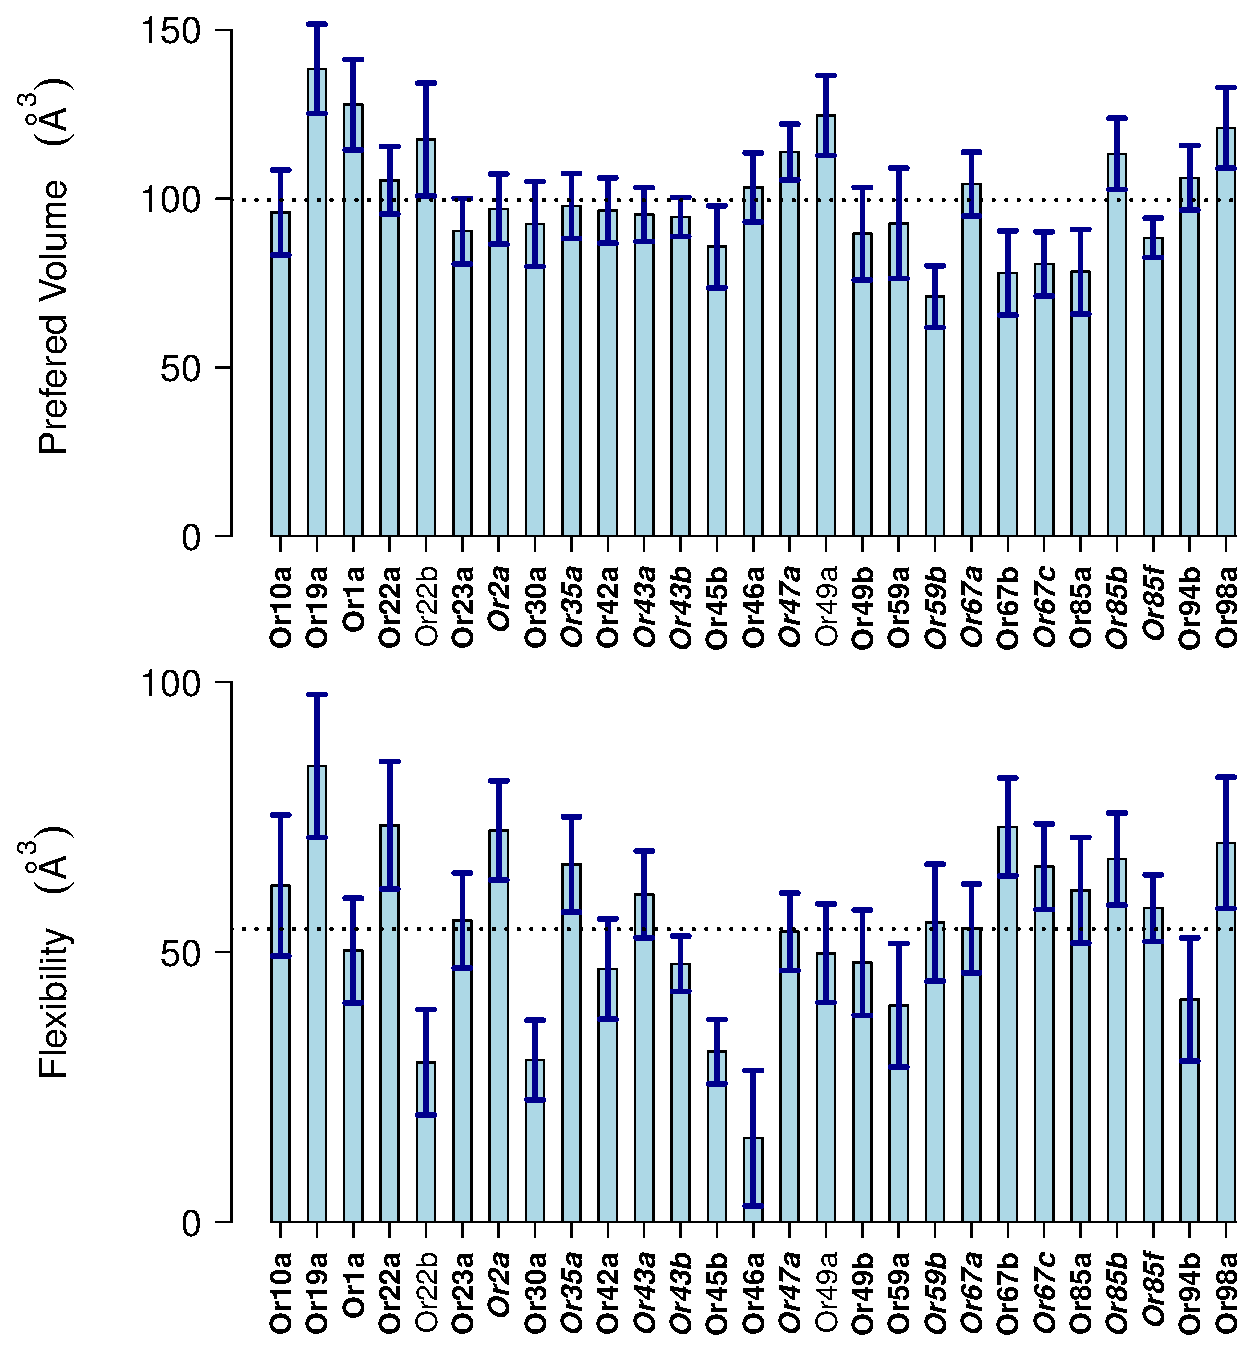
\includegraphics[width= 0.85  \textwidth]{vol-mean-std}
	\caption{The preferred volumes of \numberofreceptors OR, $v_n$ (top). 
		and their flexibilities $\sigma_n$ (down). 
		The error bars were calculated using Jack-Knife method. 
		Some ORs like Or59b, Or67a and  Or85a preferred smaller molecules, 
		but some others like Or19a,  Or1a and  Or49a preferred larger molecules.
		Some ORs like Or46a,  Or22b and Or30a were volume  selective, 
		but some others like Or19a,  Or67b and  Or22a responded to broader range of molecular volumes.
		}
		\label{fig:preferred_volume}
\end{figure}


\begin{figure}
% do not touch this fig.
	\centering
	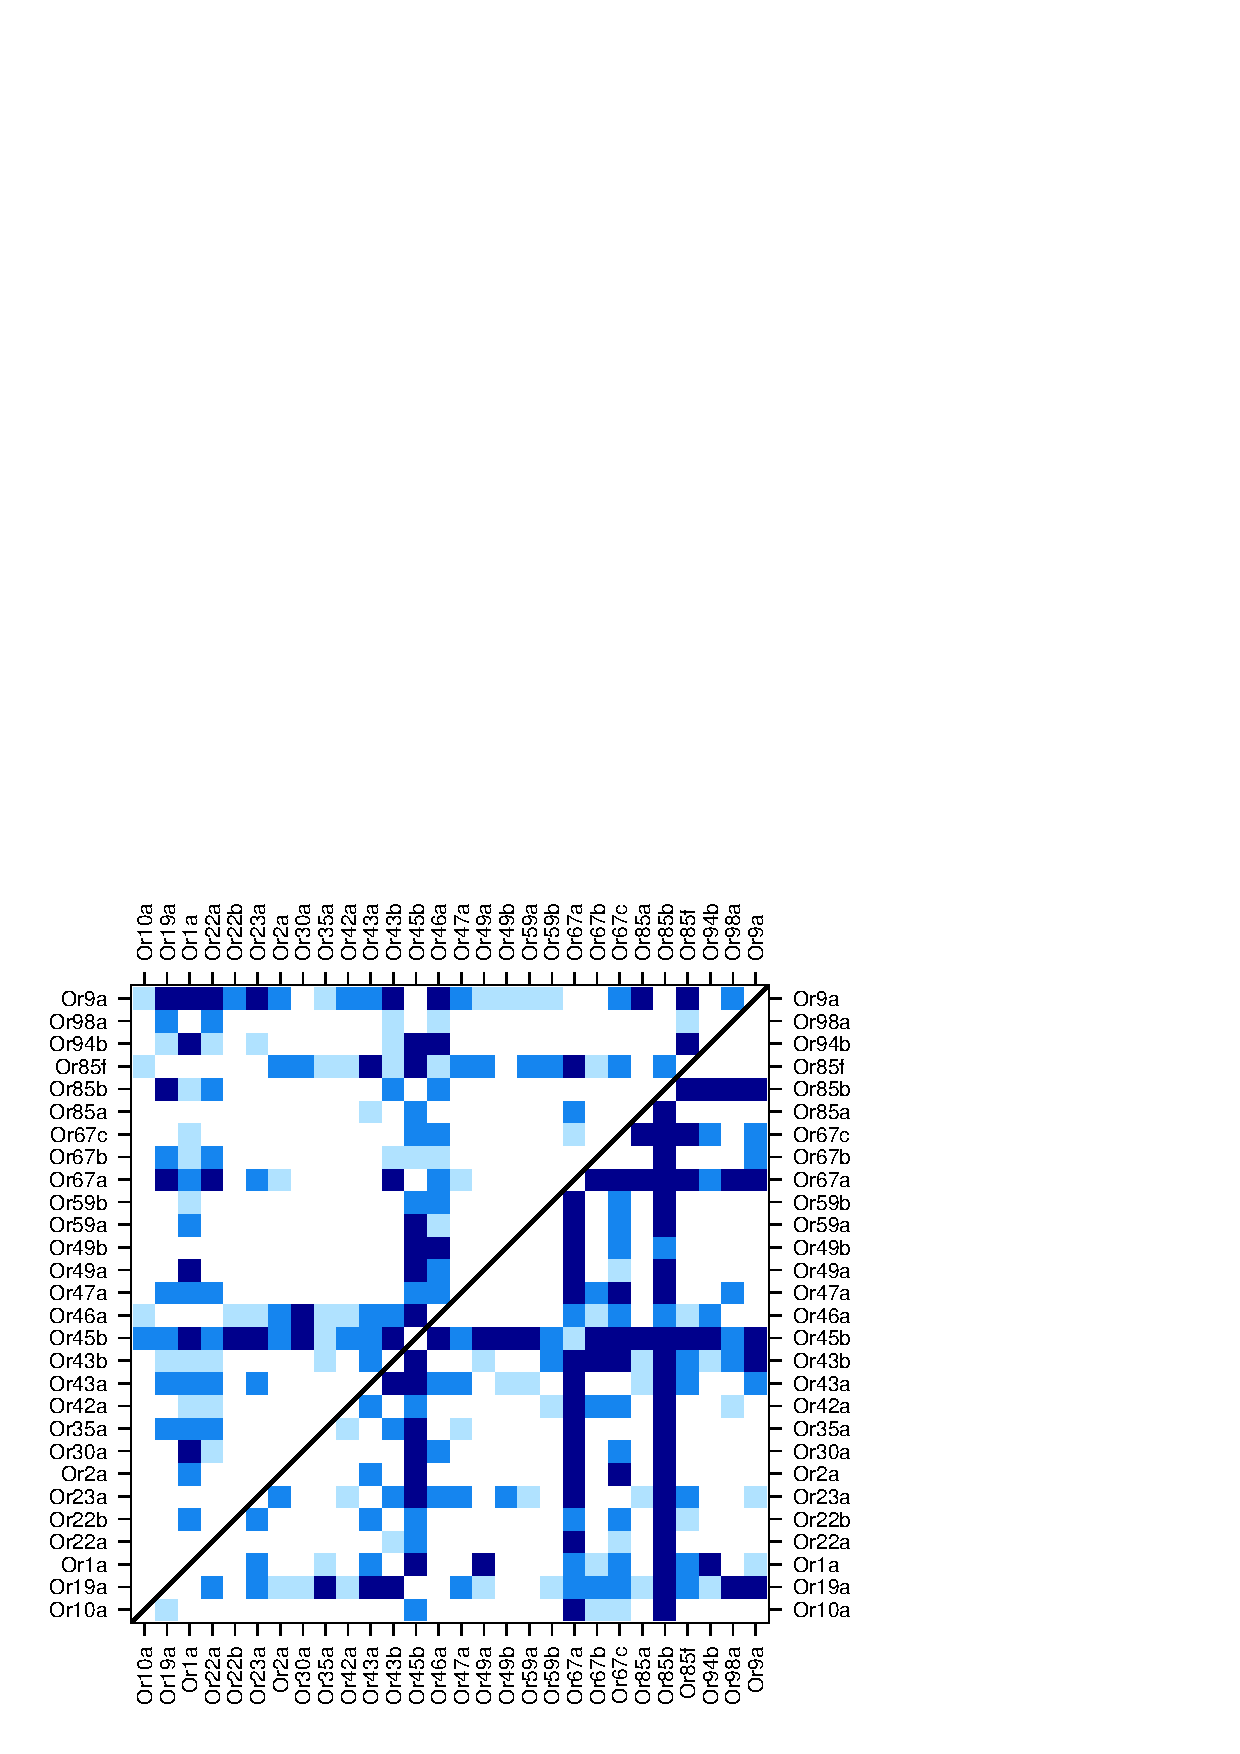
\includegraphics[width= 0.75 \textwidth]{pair-pval}
	\caption{Pairs of ORs that differed significantly in their binding-pocket's volume (upper triangle) and flexibility (lower triangle).
			All blue shades have p-value of less than 0.05, 
			two darker shades have FDR corrected p-values of less than 0.05 and the darkest shade has Bonferroni corrected p-value of less than 0.05.}
	\label{fig:p-values}
\end{figure}

%but, to be sure, we also put them in a test. 
%After calculating function $f_n(v)$ for each odorant receptor, we can calculate $\psi_{nm}$ of the equation \ref{eqn:factors}.
%If $\psi_{nm}$ is independent of molecular volumes, it means that the assumptions where justified.

The relation between molecular volumes and response of ORNs was evident (Fig.~\ref{fig:vol-res}). 
The function $f_n(v)$ could be considered as the tuning curve of OR $n$ in response to molecular volumes (Fig.~\ref{fig:vol-res}). 
Each OR had a preferred molecular volume $v_n$ and shows some flexibility $\sigma_n$. 
The calculated $f_n(v)$s are in  Fig.~\ref{fig:vol-res}. 
It includes \numberofreceptors ORs, 
which showed a significant dependence to molecular volume of odorants in their response (p-value $<0.05$). 
The flexibility of a receptor may affect the narrowness or broadness of it tuning curve, 
but we did not see any significant relation.

From the results of \numberofreceptors ORs, 
\bonferroni of them were significant according to Bonferroni correction (OR name in black), 
\fdr of them were significant according to FDR correction (OR name in gray), 
and the rest (\nocorrection ORs, name in light gray), 
only satisfied the criteria of p-value $<0.05$, without any corrections.
Considering the FDR correction, 
nearly half of ORs (\fdr / 60 ) showed significant sensitivity toward molecular volumes. 
The other half could be sensitive to molecular volume as well, 
but the current evidence are not enough and more experiments are necessary. 

\begin{figure}
% do not touch this fig.
	\centering
	\includegraphics[width= 0.75 \textwidth]{vol-res-Or82a.eps}
	\caption{(left) Or82a including Geranyl acetate (the outlier) did not confirm our theory with a p-value of 0.55, but when Geranyl acetate was removed from the data, 
	Or82a confirmed our model with a Bonfrreni corrected p-value of 0.03 (right).}
	\label{fig:Or82a}
\end{figure}
One interesting case in this regard was Or82a, that did not fit to our theory. 
It binds to Geranyl acetate much better than any other molecule. 
When we removed Geranyl acetate from the data, suddenly Or82a became a perfect fit with a Bonferroni corrected p-value of 0.03 (Fig. \ref{fig:Or82a}). 
This makes the underlying interaction between Geranyl acetate and Or82a, a special case that needs more investigations.

%\begin{table}
%\begin{center}
%    \begin{tabular}{ | l | l | l |l |}
%    \hline
%     &  $p_{value} < 0.05$ & FDR & Bonferroni \\ \hline
%     {\small Receptors are sensitive to molecular volume} &  28 &  26 & 11\\ 
%     $v_{n_1} = v_{n_2}$&  21 & 23 & 38\\ \hline
%    \end{tabular}
%\end{center}
%\caption{Times that the null hypothesis has been rejected, according to different method}
%\end{table}
The parameters of $f_n(v)$, $v_n$ and $\sigma_n$ are in Fig. \ref{fig:preferred_volume}.
Figure \ref{fig:preferred_volume} demonstrate that the molecular volume preference of ORs were different (top). 
and the flexibility of ORs were also different (bottom).
To backup these claims, 
we estimated the p-values of having different volume preference and flexibility for each pairs of \numberofreceptors ORs
(Fig.~\ref{fig:p-values}). 
From all possible 378 pairs, 
when comparing the volume preferences, 
133 had a p-value of less than 0.05, 
this number reduced to 89 after using FDR and further reduced to 32 using Bonferroni correction.
When comparing flexibilities, 
the numbers were 168, 134 and 77 respectively. 
The union of these two set confirmed that 226 (p-value $<0.05$), 171 (FDR corrected), and 91 (Bonferroni corrected) pairs of ORs showed distinct differences in their binding-pocket characteristics.

The diversity of ORs is important in perceiving the quality of smells. 
In a hypothetical experiment, 
assume that every characteristic of odorant molecules are the same but their molecular volume.
If all ORs  have the same preferred volume and flexibility, 
any change in the molecular volume will change only the intensity of smell not its quality.
Here we showed that ORs  had different preferred volumes and flexibilities, 
so any change in the molecular volume of an odorant results in a different combinatorial encoding which affects the quality of perceived smell as well its intensity.
This agreed with the work of M. Zarzo: larger molecules  smell better~\cite{zarzo2011}.
That might describe the difference in the smell of methanol, ethanol, propanol and butanol. 
Methanol smells pungent, ethanol smells pleasant and winy, propanol and butanol smell like ethanol except butanol has a little banana like aroma.
We suggested that the molecular volume affects the combinatorial encoding, 
and the combinatorial code determines the quality of odorants.

Here we showed that the responses of ORNs are related to the molecular volume of odorants, 
apart from that, it is not clear which other features of molecules are measured by ORs. 
There are many works that try to connect the physio-chemical properties of molecules to the evoked neural response or perceived smells.
But the non-linear volume dependence (Eq. \ref{eqn:factors} and Eq. \ref{eqn:volume-dependence})  
may mask important relations between molecules and neural responses.
When $f_n(v)$ is close to zero, 
the value of $\psi_{nm}$ does not matter. 

We predicted odorants with a molecular volume on the tails of $f_n(v)$ goes undetected, 
regardless of any other physio-chemical properties that they may have. 
This prediction can be confirmed in further experiments. 

To better study $\psi_{nm}$ of an OR, 
it is better to have many data points and those data points are better to be around the preferred volume of the OR.
But this is not the case in current data. 
For many ORs, 
most data points are on the tails of $f_n(v)$, which is close to zero.
We suggested the best selection of odorants for each of \numberofreceptors studied ORs 
(see Venn diagram in Fig.~\ref{fig:odorant-suggest} and supplemental file proposed-odorants.csv), 
saving time and expenses of future experiments. 

%After gathering enough data, 
%by considering the effect of molecular volume on the response of odorant receptor neurons, 
%one might discover more subtle dependence between other molecular features and neural responses, 
%by investigating $\psi_{nm}$, 
%which otherwise would be masked by this non-linear relation $f_n(v)$.

We also predicted some {\it in-vivo} structural aspects of  the binding-pocket of ORs:
the preferred volume of each OR results from the volume of the binding-pocket,
the flexibility of an OR results from the rigidity or flexibility of the binding-pocket; 
%Therefore, our results provides information about both structural and dynamical properties of odorant receptors in Drosophila. 
These data added some constrains over the 3d structure of ORs, 
which might help the prediction and calculation of 3d structure of these proteins. 

The method of this work can be combined with mutagenesis as well. 
Some genes of an OR are mutated, 
then its response to a selection of molecules are measured and finally the preferred volume and flexibility are calculated.
In this way we can understand which amino acids of the OR contribute to the volume and flexibility of the binding-pocket, 
as well as affecting the function of the ORs.

In this work, we have overlooked many facts, 
because the nature of the problem is inherently complex and otherwise would not be feasible to study. 
There are many factors that affects the concentration of odorant molecules at the close to the receptors, 
like molecular mass, vapor pressure, solubility in water, sensillum lymph and its odorant binding proteins (lush) \cite{}. 
It is difficult to control them in the current experimental apparatus and they make the model very complex with many sets of parameters. 
Using experimental paradigm like Luciferase Assay as used to study human olfactory systems \cite{human olf}, 
may provide valuable complementary information to our simple model. 
We expect these factors have minimal effect on smaller molecules, 
because they evaporate easily and solve in water well and they might not need the help of odorant binding protein, 
so we can be confident about the lack of response to small molecules more than what we can say about larger molecules. 

\begin{figure}
\centering
	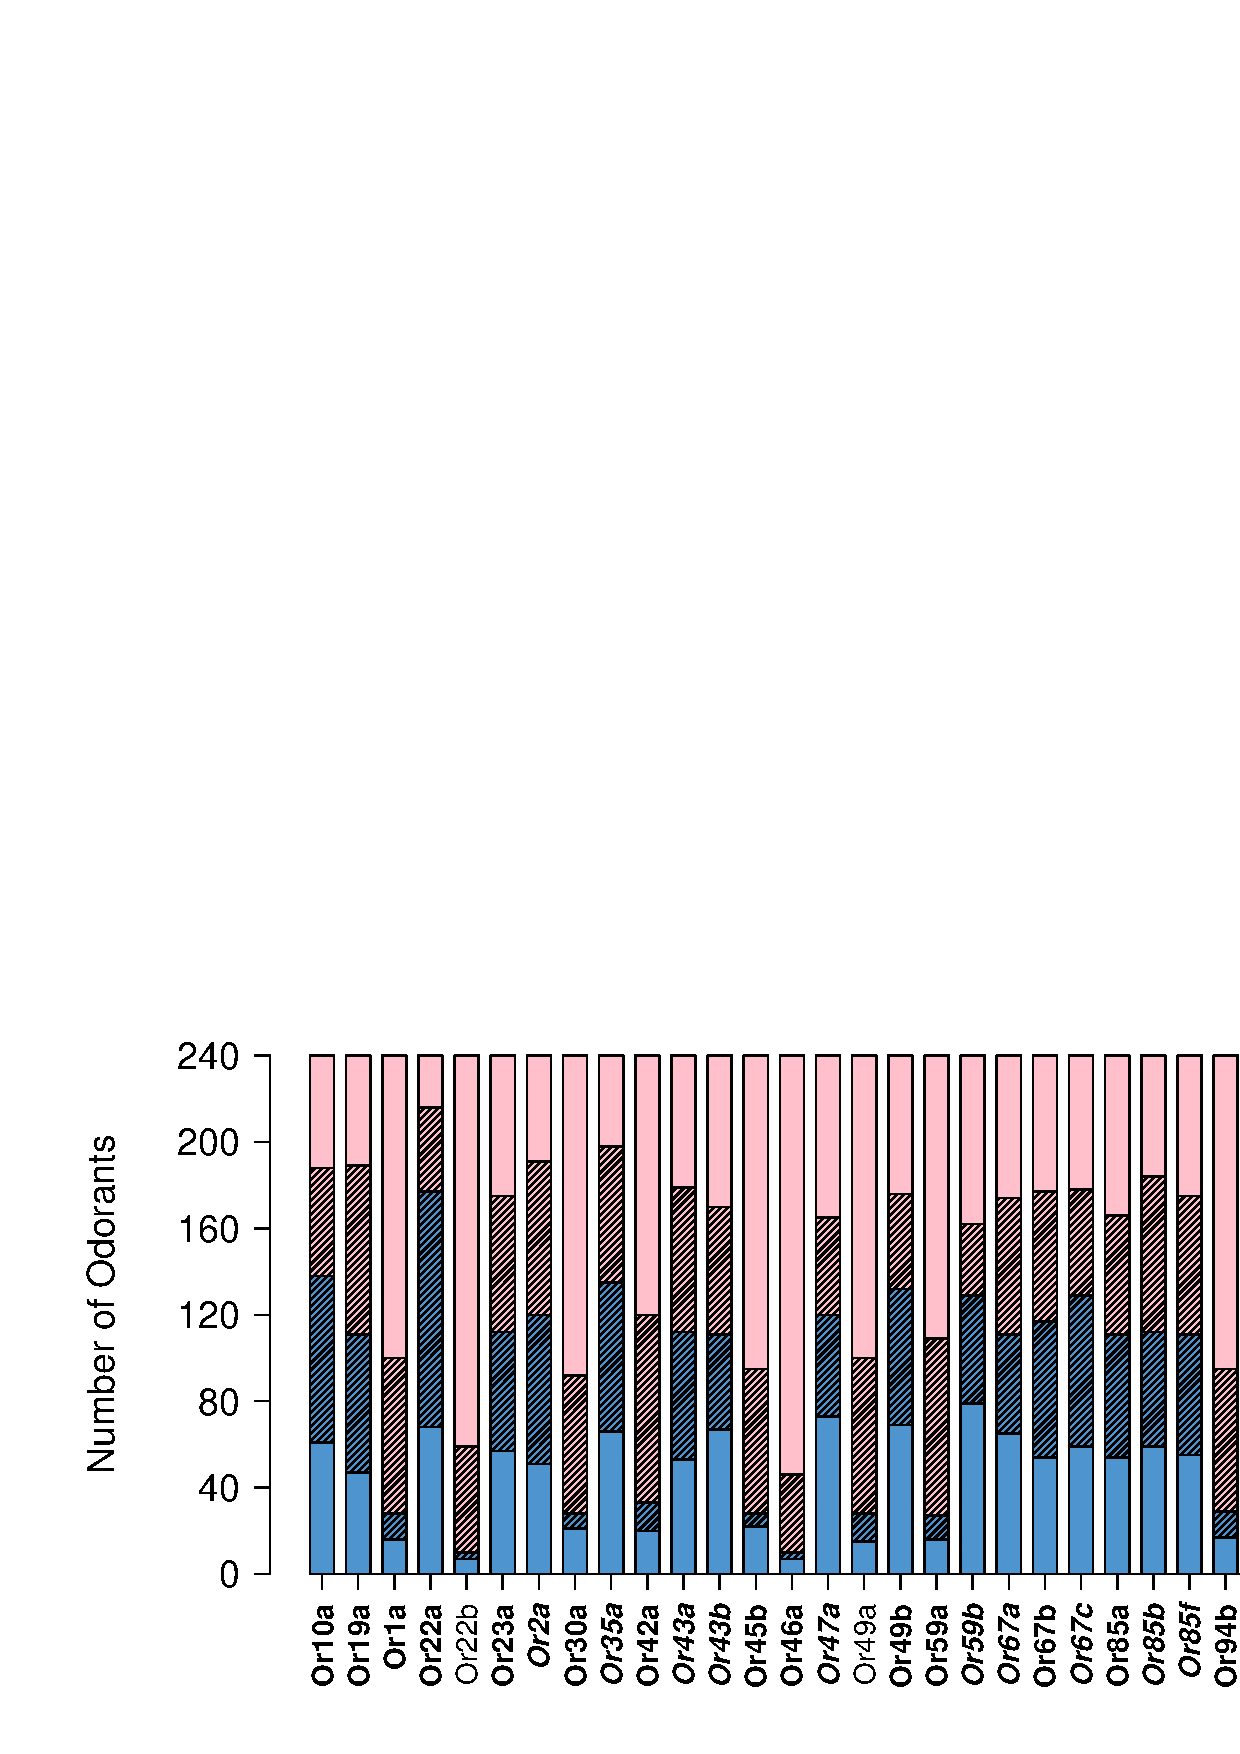
\includegraphics[width=\textwidth]{odorant-suggest}
	\caption{Venn diagram of DoOR database and our suggested important odorants of each OR.
			The database includes 240 molecules, 
			some are used to study an OR (blue areas), 
			and data for the rests are not available (pink).
			The hatched area are odorants with molecular volume close to the preferred volume of each OR
			($v_n \pm \frac{\sigma}{2}$).
			We already know the neural response of hatched blue areas, 
			but the hatched pink odorants could be the target of future experiments, we predict the rest give only zeros.
			}
	\label{fig:odorant-suggest}
\end{figure}

\section*{Conclusion}

We showed that molecular volume was an important factor, 
but not the only one that determined the response of olfactory receptor neurons (ORNs). 

We hypothesized that this was resulted from the volume of binding-pocket of odorant receptors (ORs) and its flexibility. 
We predicted the actual \textit{in-vivo} volume and flexibility of the binding-pockets of ORs. 
The results are in supplemental file volume-profiles.csv and they can be verified when the 3D structure is resolved, 
or more experimental results are available. 

Now that we know how much of the variance in the response of ORN was resulted from molecular volume, 
it is possible to study the effect of other parameters.

We approximated a molecule with a rigid isotropic sphere of given volume, 
so our model does not say anything about shape \cite{}, vibrational mode \cite{}, chirality \cite{some and this: Dissipative Vibrational Model for Chiral Recognition in Olfaction} or many other interestig properties of a molecule.
Actually our method and results are a starting point to other factors. 
A simple improvement that can be made on the model is to include anisotropy of the molecules, 
simply by modeling  them as ellipsoids.

Approximating $f_n(v)$ and $g(v)$ with a Gaussian function makes the mathematical formulation simple and readable. 
But a semi-infinite function may be a better choice for molecular volumes which can not have negative values.

Although this work was on the data of \textit{Drosophila}, 
we expect that the general principles and methodologies of this work hold for vertebrates as well, 
we are working to apply the same method to data of human olfactory receptors \cite{}.

%There are two main assumption in this work: 
%First we assumed that the response of an OR could be factorized into two terms, 
%according to (\ref{eqn:factors}).
%Second, we assumed that the volume dependence factor $f_n(v_m)$ in (\ref{eqn:factors}) 
%had a Gaussian form (Eq. \ref{eqn:volume-dependence}).
%Considering the physics and chemistry behind the binding-process (Fig. \ref{fig:binding-pocket}), 
%and the neural responses (Fig. \ref{fig:vol-res}), 
%these assumptions were logical. n


%Our work can be improved in many ways, we can consider the anisotropy of molecular shape, and we can improve the approximation of $f_n(v)$. 

%Molecules have complex shapes, 
%in this work we have used the simplest possible approximation, 
%we approximated a molecule with a sphere, 
%kept only its volume and discarded any other spatial complexity. 
%This can be improved by approximating a molecule with an ellipsoid, 
%In this way more spatial details will be taken into account. 

\section*{Acknowledgments}
We are especially grateful to B. N. Araabi, S. Aghvami, N. Doostani and Shima Seyed-allaei for the careful reading of the manuscript.
%; and P. Carloni for the fruitful discussion.

\printbibliography

%\bibliography{binding-pocket}

%\bibliographystyle{Science}


\section*{Contributions}

M.S. and H.S. equally contributed to the design of the study. H.S. developed the mathematical framework, M.S. prepared the data and analyzed them. H.S. made Fig. 1 and M.S. produced all other figures. H.S. composed the article and M.S. managed the bibliography. Both authors has reviewed the manuscript.

\section*{Competing interests}
The authors declare no competing financial interests.


\end{document}
